\documentclass[11pt]{article}

\usepackage[margin=1in]{geometry}
\usepackage{amsmath, amsthm, amssymb, amsfonts}
\usepackage{mathtools}
\usepackage{bm}
\usepackage{graphicx}
\usepackage{booktabs}
\usepackage{microtype}
\usepackage{enumitem}
\usepackage{natbib}
\usepackage{xcolor}
\usepackage{hyperref}
\hypersetup{colorlinks=true, linkcolor=blue!50!black, citecolor=blue!50!black, urlcolor=blue!50!black}

% Theorem environments
\theoremstyle{plain}
\newtheorem{theorem}{Theorem}[section]
\newtheorem{proposition}[theorem]{Proposition}
\newtheorem{lemma}[theorem]{Lemma}
\newtheorem{corollary}[theorem]{Corollary}
\theoremstyle{definition}
\newtheorem{definition}[theorem]{Definition}
\newtheorem{assumption}[theorem]{Assumption}
\theoremstyle{remark}
\newtheorem{remark}[theorem]{Remark}
\newtheorem{example}[theorem]{Example}

% Shortcuts
\newcommand{\R}{\mathbb{R}}
\newcommand{\Z}{\mathbb{Z}}
\newcommand{\N}{\mathbb{N}}
\newcommand{\C}{\mathbb{C}}
\newcommand{\E}{\mathbb{E}}
\newcommand{\Var}{\mathrm{Var}}
\newcommand{\norm}[1]{\left\lVert#1\right\rVert}
\newcommand{\abs}[1]{\left\lvert#1\right\rvert}
\newcommand{\inner}[2]{\left\langle#1,#2\right\rangle}
\DeclareMathOperator*{\argmin}{arg\,min}
\DeclareMathOperator*{\argmax}{arg\,max}
\newcommand{\method}{polynomial hint preconditioning}
\newcommand{\Method}{Polynomial hint preconditioning}
\newcommand{\HD}{\textsf{HD10}}
\newcommand{\Baseline}{\textsf{Baseline}}
\newcommand{\Zero}{\textsf{Zero}}
\newcommand{\Dup}{\textsf{Duplicate}}

\title{\textbf{Polynomial Hint Preconditioning for\\Universal Time Series Forecasting}}
\author{
  Jerry Han \\[0.5em]
  \small Department of Mathematics \\
  \small Program in Statistics and Machine Learning \\
  \small Princeton University \\[0.5em]
  \small Advisor: Prof.\ Elad Hazan \\
  \small Second Reader: Prof.\ Amit Singer
}
\date{Spring 2026}

\begin{document}
\maketitle

\begin{abstract}
\noindent
Patch-based transformer architectures for universal time series forecasting segment the input into fixed-length patches and embed each patch independently, creating a \emph{cross-patch information bottleneck}: temporal patterns spanning multiple patches must be recovered entirely through attention. Drawing on the recent theoretical framework of universal sequence preconditioning~\citep{marsden2024universal}, which shows that polynomial transformations of a sequence reduce the spectral complexity faced by online predictors of linear dynamical systems, we propose \textbf{\method} for patch-based transformers. We apply a fixed Chebyshev polynomial FIR filter to the raw time series and concatenate the result as an auxiliary input channel, injecting cross-patch temporal information with negligible parameter overhead ($12\,$K parameters, $0.11\%$ of the model). Two lines of justification underpin the choice of Chebyshev polynomials: (i) the classical equioscillation theorem of Chebyshev, which characterises the monic degree-$d$ polynomial of minimal supremum norm on $[-1,1]$; and (ii) the regret-reduction theorems of Marsden and Hazan, which show that such preconditioners yield sublinear, hidden-dimension-independent regret bounds for marginally stable linear dynamical systems. We analyse our specific filter's frequency response in closed form, prove a stability lemma, and validate the theoretical predictions on synthetic linear dynamical system trajectories and on the GIFT-Eval benchmark of 97 dataset--horizon configurations. Across 5 seeds and 485 paired comparisons, our method improves geometric mean MASE by $2.9\%$ over the Moirai-2 Small baseline ($p < 10^{-15}$), winning 329 of 485 comparisons after Holm--Bonferroni correction at $\alpha=0.05$. Controlled capacity experiments confirm that the improvement is driven by polynomial content rather than extra parameters: duplicating the input as a second channel \emph{hurts} performance ($44.7\%$ win rate), while a zero channel is essentially neutral. At $100$K training steps, the improvement grows to $3.9\%$. We report Holm--Bonferroni-corrected $p$-values, bootstrap confidence intervals, and an analysis of which dataset frequency-structure characteristics predict the size of the improvement, testing the spectral hypothesis implied by the theory.
\end{abstract}

\section*{Acknowledgments and Contributions}

I am deeply grateful to my advisor, Prof.\ Elad Hazan, for suggesting the connection between universal sequence preconditioning and patch-based time series foundation models, and for numerous conversations that shaped the direction of this work. I thank Prof.\ Amit Singer for serving as second reader and for feedback on the mathematical exposition. Any errors are my own.

\paragraph{Individual contributions.}
The theoretical formulation, experimental design, implementation, and writing presented in this paper are my individual work. The framework of universal sequence preconditioning as applied to online prediction of linear dynamical systems is due to \citet{marsden2024universal}; the extension of that framework to patch-based transformer forecasting, the specific filter design, the empirical methodology, the statistical analysis, and all figures and tables were developed by me. Computational experiments were run on the Princeton Research Computing cluster.

\paragraph{Relation to workshop submission.}
An abridged 4-page version of the empirical portion of this work was submitted concurrently to the ICML 2026 Workshop on Foundation Models for Structured Data (FMSD); the workshop is non-archival. This Junior Paper contains substantially expanded mathematical analysis, additional theoretical results, and additional empirical validation (synthetic linear dynamical system experiments and a spectral-correlate analysis) not present in the workshop submission.

\tableofcontents

%==============================================================================
\section{Introduction}
%==============================================================================

Universal time series forecasting~\citep{woo2024unified, liu2024moirai2, das2024decoder, ansari2024chronos, goswami2024moment, auer2025tirex} has emerged as a pretraining paradigm for transformer-based models trained on heterogeneous corpora that span frequencies from sub-hourly to yearly, and whose behaviour at inference time is expected to transfer across unseen domains without task-specific fine-tuning. A growing body of models---Moirai, TimesFM, Chronos, MOMENT, TiRex---shares a common architectural primitive with PatchTST~\citep{nie2023patchtst} and Vision Transformer~\citep{dosovitskiy2021image}: the input sequence is segmented into non-overlapping patches of length $P$, each patch is projected to a $d$-dimensional embedding independently, and interactions across patches are mediated entirely by self-attention. This design yields substantial gains in throughput relative to token-level transformers, but it introduces what we call the \emph{cross-patch information bottleneck}: each patch embedding, before the first attention layer, encodes only $P$ time steps, so temporal correlations whose natural scale exceeds $P$ (e.g., daily periodicities in $15$-minute data, spanning $96$ steps or six patches at $P=16$) must be discovered end-to-end by the attention mechanism. Smaller models, with fewer attention heads and layers, are especially constrained.

\paragraph{Our intervention.}
We propose \textbf{\method{}}, a simple architectural change that alleviates the cross-patch bottleneck at constant parameter cost. Given the input sequence $x[t]$, we compute a \emph{hint channel} by applying a fixed finite-impulse-response filter
\begin{equation}
    h[t] = (p(B_s) x)[t] = \sum_{k=0}^{d} a_k \, x[t - k s],
    \label{eq:hint-intro}
\end{equation}
where $B_s$ is the shift-by-$s$ operator $(B_s x)[t] = x[t-s]$, the polynomial $p(z) = \sum_{k=0}^d a_k z^k$ is a degree-$d$ polynomial with coefficients derived from the monic Chebyshev polynomial $\tilde{T}_d$, and the stride $s$ is set equal to the patch size $P$. The hint channel is concatenated with the target and observation-mask channels before the initial per-patch projection. Only the width of this first projection grows; the transformer encoder is unchanged. For $d = 4$ and $s = P = 16$, the hint reduces to
\[
    h[t] = x[t] - x[t - 2 P] + \tfrac{1}{8} x[t - 4 P],
\]
which injects information from two and four patches in the past into each current-patch embedding \emph{before} the first attention layer---at a cost of $12$K extra parameters, or $0.11\%$ of the Moirai-2 Small model.

\paragraph{Mathematical motivation.}
Two threads of mathematics motivate this design. The first is classical: the \emph{Chebyshev equioscillation theorem} states that among all monic polynomials of degree $d$ on the interval $[-1,1]$, the monic Chebyshev polynomial $\tilde{T}_d$ uniquely attains the minimal supremum norm, which equals $2^{1 - d}$~\citep{davis1975interpolation}. Consequently, any degree-$d$ transformation of a sequence whose power is spectrally concentrated on a normalized frequency interval is best compressed---in the uniform-norm sense---by Chebyshev coefficients. The second thread is modern: \citet{marsden2024universal} show that, within the framework of online prediction of linear dynamical systems (LDS), applying a polynomial $p(B)$ to the target sequence is \emph{equivalent} to applying $p(A)$ to the hidden transition matrix $A$, and they prove that Chebyshev and Legendre preconditioners yield the first sublinear and hidden-dimension-independent regret bounds for systems with marginally stable, possibly asymmetric, transition matrices. While patch-based transformers are not literally online predictors of LDSs, the spectral intuition transfers: a polynomial preconditioner redistributes the signal's energy across frequency bands in a way that disentangles long-scale correlations, and Chebyshev coefficients achieve the best worst-case redistribution within the monic degree-$d$ family.

\paragraph{Empirical evidence.}
We retrain the Moirai-2 Small encoder~\citep{liu2024moirai2} (11.4M parameters, six transformer blocks, $P=16$) on the LOTSA corpus~\citep{woo2024unified} for $10$K and $100$K optimizer steps, comparing four conditions: a standard \Baseline{}, a capacity-matched \Zero{} control (auxiliary channel filled with zeros), a capacity-matched \Dup{} control (auxiliary channel = copy of input), and our method \HD{} (Chebyshev $d=4$, stride $16$, $10\%$ hint dropout). On the $97$-configuration GIFT-Eval benchmark~\citep{vijay2024gifteval}, at context length $4{,}000$ and with five random seeds, \HD{} improves geometric-mean MASE by $2.9\%$ at $10$K steps ($p<10^{-15}$, sign test on $485$ paired comparisons; Holm--Bonferroni-corrected across all evaluated methods) and by $3.9\%$ at $100$K steps. Importantly, the \Dup{} capacity control \emph{hurts} performance ($44.7\%$ win rate) and \Zero{} is neutral ($54\%$, $p=0.042$ unadjusted), identifying the polynomial content---not the extra parameters---as the source of the gain. Cross-domain analysis confirms the spectral hypothesis: gains are largest on high-frequency domains (transport, energy) whose natural time scales align with the filter's lookback structure, and negligible on weather and healthcare where the dominant variations occur at scales either much shorter or much longer than our stride-$16$ filter.

\paragraph{Contributions and Outline.}
The remainder of this paper develops the following contributions:
\begin{enumerate}[leftmargin=1.5em, topsep=0.2em, itemsep=0.2em]
  \item A rigorous statement (Section~\ref{sec:preliminaries} and Section~\ref{sec:precondition}) of the mathematical framework of universal sequence preconditioning, specialized from online LDS prediction to patch-based transformer forecasting, including the frequency-response analysis of our specific filter.
  \item A self-contained proof sketch (Section~\ref{sec:chebyshev}) of the Chebyshev equioscillation theorem and its implications for polynomial preconditioning, and a closed-form derivation of the frequency response $H(e^{j\omega})$ of our hint filter (Theorem~\ref{thm:freq-response}).
  \item A stability lemma (Lemma~\ref{lem:stability}) establishing that the preconditioning operation preserves bounded variance and is hence BIBO-stable, relevant for practical numerical behavior.
  \item An empirical validation (Section~\ref{sec:empirical}) on: (a) synthetic marginally-stable linear dynamical systems, demonstrating that the empirical forecast-error reduction matches the theoretical prediction; (b) the GIFT-Eval benchmark, with extensive capacity-control ablations and a spectral-correlate analysis that tests the frequency-response hypothesis dataset-by-dataset.
  \item A rigorous statistical methodology section (Section~\ref{sec:stats}) presenting multiple-testing-corrected significance tests, bootstrap confidence intervals, and effect sizes, supporting the paper's inferential claims and contextualizing the size of the observed improvement.
\end{enumerate}

%==============================================================================
\section{Preliminaries}
\label{sec:preliminaries}
%==============================================================================

We review three strands of background that our development relies on: linear dynamical systems and their forecasting, patch-based transformer architectures, and Chebyshev approximation theory. A reader familiar with any of these may skim the corresponding subsection.

\subsection{Linear Dynamical Systems and Sequence Forecasting}

A \emph{linear dynamical system} (LDS) with hidden dimension $m$ and observation dimension $n$ is specified by matrices $A \in \R^{m \times m}$, $C \in \R^{n \times m}$, and sequences of process noise $w_t \in \R^m$ and observation noise $e_t \in \R^n$. The system evolves according to
\begin{equation}
    h_{t+1} = A h_t + w_t, \qquad y_t = C h_t + e_t, \qquad t \in \Z_{\geq 0},
    \label{eq:lds}
\end{equation}
with initial state $h_0 \in \R^m$. In the \emph{online prediction} problem, a learner sees $y_1, y_2, \ldots$ sequentially and at each step $t$ outputs a prediction $\hat y_{t+1}$ of the next observation; performance is measured by the cumulative regret
\[
    \mathrm{Regret}_T = \sum_{t=1}^T \ell(\hat y_{t+1}, y_{t+1}) - \min_{\text{class}} \sum_{t=1}^T \ell(\tilde y_{t+1}, y_{t+1}),
\]
where $\ell$ is a convex loss (typically squared error) and the minimum ranges over a comparator class such as linear functions of $y_{1:t}$.

The \emph{spectral radius} $\rho(A) = \max_i |\lambda_i(A)|$ of the transition matrix controls the forecastability of the system. When $\rho(A) < 1$ (strictly stable), the memory of the system decays geometrically and classical regret bounds of order $O(\sqrt{T} \, \mathrm{poly}(m))$ are available~\citep{hazan2017learning}. When $\rho(A) = 1$ (marginally stable, e.g., pure sinusoids or integrated processes), standard bounds degrade, with the dependence on $m$ often becoming linear or worse.

\subsection{Patch-based Transformer Forecasting}

A patch-based transformer forecaster~\citep{nie2023patchtst, woo2024unified} proceeds as follows. Given a univariate history $x[1{:}T]$, partition it into non-overlapping patches $\mathbf{p}_i = (x[(i{-}1)P{+}1], \ldots, x[iP])$ of length $P$ for $i=1, \ldots, T/P$. A per-patch projection $W \in \R^{d \times P}$ maps each patch to an embedding $\mathbf{e}_i = W \mathbf{p}_i + b \in \R^d$. These embeddings are summed with positional encodings and fed to a standard transformer encoder, whose output predicts future patches (often jointly across a set of quantile levels via a specialized head; see~\citealp{liu2024moirai2}). Two features of this architecture are salient for our development:
\begin{itemize}[leftmargin=1.5em, itemsep=0.1em, topsep=0.2em]
    \item \emph{Cross-patch information must be learned via attention.} Before the first self-attention operation, $\mathbf{e}_i$ is a function of $\mathbf{p}_i$ alone; it contains no information about $\mathbf{p}_{i-1}$, $\mathbf{p}_{i+1}$, or more distant patches.
    \item \emph{The per-patch projection $W$ is narrow.} In Moirai-2 Small, $P = 16$ and $d = 384$, so the projection has $P \cdot d = 6{,}144$ parameters (with a small additive bias and a residual structure, the effective count is $\approx 10$K). Altering the \emph{input} to this projection is therefore cheap; altering downstream layers is not.
\end{itemize}

\subsection{Chebyshev Polynomials}
\label{sec:chebyshev-prelim}

The \emph{Chebyshev polynomials of the first kind}, denoted $T_d(x)$ for $d \in \Z_{\geq 0}$, are defined by the recurrence
\begin{equation}
    T_0(x) = 1, \quad T_1(x) = x, \quad T_{d+1}(x) = 2 x \, T_d(x) - T_{d-1}(x),
    \label{eq:cheb-recurrence}
\end{equation}
or equivalently by the trigonometric identity $T_d(\cos \theta) = \cos(d \theta)$. The first several polynomials are $T_2(x) = 2x^2 - 1$, $T_3(x) = 4x^3 - 3x$, $T_4(x) = 8x^4 - 8x^2 + 1$. The leading coefficient of $T_d$ is $2^{d-1}$, so the \emph{monic Chebyshev polynomial} is $\tilde T_d(x) = T_d(x) / 2^{d-1}$. For $d = 4$,
\[
    \tilde T_4(x) = x^4 - x^2 + \tfrac{1}{8}.
\]

Chebyshev polynomials possess several extremal properties; one of the most celebrated is the \emph{equioscillation property} underlying the approximation theorem we state in Section~\ref{sec:chebyshev}.

%==============================================================================
\section{Universal Sequence Preconditioning}
\label{sec:precondition}
%==============================================================================

We now review the framework of \citet{marsden2024universal}, which motivates our filter design, and specialize it to patch-based forecasting.

\subsection{Polynomial Preconditioning of LDS Observations}

Consider an LDS as in~\eqref{eq:lds} with noise terms neglected for exposition. Then $y_t = C A^t h_0$ and the $d$-step differenced or preconditioned observation
\[
    \tilde y_t \;=\; (p(B) y)[t] \;=\; \sum_{k=0}^d a_k y_{t-k} \;=\; C \Big( \sum_{k=0}^d a_k A^{-k} \Big) A^t h_0 \;=\; C \, p(A^{-1}) A^t h_0,
\]
where $B$ denotes the backshift operator and $p(z) = \sum_{k=0}^d a_k z^k$. Reversing the polynomial (equivalently, working with the reciprocal polynomial $p^*(z) = z^d p(1/z)$) gives the cleaner identity
\[
    \tilde y_t \;=\; C \, p^*(A) A^{t-d} h_0,
\]
so that preconditioning in observation space corresponds to \emph{multiplying the hidden state's dynamics by $p^*(A)$}. If the eigenvalues of $A$ lie in an interval $[-\rho, \rho] \subset \R$ (real spectrum), then for any monic degree-$d$ polynomial $q$,
\[
    \rho\big( q(A) \big) \leq \max_{\lambda \in [-\rho, \rho]} \abs{ q(\lambda) },
\]
and the right-hand side is \emph{minimized over monic $q$ of degree $d$} by $q = \rho^d \, \tilde T_d(\,\cdot\,/\rho)$---this is the content of the classical Chebyshev minimax theorem (Theorem~\ref{thm:chebyshev-minimax} below). Preconditioning by the Chebyshev-derived polynomial therefore compresses the effective spectral radius seen by a downstream online predictor, yielding the regret-reduction theorems of~\citet[Thms.~3 and~5]{marsden2024universal}.

\subsection{Specialization to Patch-based Forecasting}

Our setting differs from the LDS online-prediction setting in three ways: (i) the forecaster is a pretrained transformer, not an online least-squares or follow-the-regularized-leader algorithm; (ii) the data-generating process is unknown and not assumed to be a finite-dimensional LDS; (iii) rather than \emph{replacing} the target sequence by its preconditioned version, we \emph{concatenate} the preconditioned sequence as an auxiliary input channel.

Design (iii) is key. Replacing $y$ by $p(B) y$ discards the (low-frequency or unshaped) content of the original signal, which the transformer may still use; concatenation hands the model both representations and lets attention layers combine them. It also preserves the forecasting target: we precondition the \emph{input}, not the supervision signal.

Despite these differences, the spectral intuition transfers. A preconditioning filter redistributes the input's energy across frequency bands; Chebyshev coefficients achieve the minimax-optimal redistribution for a given filter degree; and a patch-based transformer facing a signal whose spectrum has been shaped to highlight multi-patch correlations is plausibly better-equipped to capture them.

%==============================================================================
\section{Theoretical Analysis}
\label{sec:chebyshev}
%==============================================================================

This section establishes three results: the classical Chebyshev minimax theorem (Theorem~\ref{thm:chebyshev-minimax}), a closed-form frequency response for our filter (Theorem~\ref{thm:freq-response}), and a stability lemma for the preconditioning operation (Lemma~\ref{lem:stability}).

\subsection{Chebyshev Minimax and the Equioscillation Theorem}

\begin{theorem}[Chebyshev Minimax; cf.\ \citealp{davis1975interpolation}]
\label{thm:chebyshev-minimax}
Among all real monic polynomials of degree $d \geq 1$, the monic Chebyshev polynomial $\tilde T_d$ uniquely minimizes $\sup_{x \in [-1,1]} \abs{q(x)}$:
\begin{equation}
    \tilde T_d \;=\; \argmin_{q \text{ monic, } \deg q = d} \; \max_{x \in [-1,1]} \abs{q(x)}, \qquad \max_{x \in [-1,1]} \abs{\tilde T_d(x)} = 2^{1-d}.
\end{equation}
\end{theorem}

\begin{proof}[Proof sketch]
The bound $\sup_{[-1,1]} \abs{\tilde T_d} = 2^{1-d}$ follows immediately from $T_d(\cos\theta) = \cos(d\theta)$, which gives $\sup_{[-1,1]} \abs{T_d} = 1$. To see uniqueness, suppose $q$ is a monic degree-$d$ polynomial with $\sup_{[-1,1]} \abs{q} < 2^{1-d}$. Consider $r = \tilde T_d - q$, which has degree at most $d - 1$ (leading terms cancel). The polynomial $\tilde T_d$ equioscillates at the $d+1$ points $\{\cos(k\pi / d)\}_{k=0}^{d}$, alternating between $\pm 2^{1-d}$; at each of these points, $r$ inherits the sign of $\tilde T_d$ (because $\abs{q} < 2^{1-d}$), so $r$ has at least $d$ sign changes on $[-1, 1]$. By the intermediate-value theorem $r$ has at least $d$ zeros, but $\deg r \leq d - 1$, a contradiction. Hence no such $q$ exists.\qedhere
\end{proof}

An immediate corollary is the spectral-compression statement used in Section~\ref{sec:precondition}:

\begin{corollary}
\label{cor:spectral-compression}
Let $A \in \R^{m \times m}$ be diagonalizable with real spectrum contained in $[-\rho, \rho]$. Then among all monic polynomials $q$ of degree $d$, the choice $q(\lambda) = \rho^d \, \tilde T_d(\lambda / \rho)$ minimizes $\rho(q(A))$, attaining the bound
\[
    \rho\big( q(A) \big) \;\leq\; \rho^d \cdot 2^{1 - d}.
\]
\end{corollary}

Corollary~\ref{cor:spectral-compression} provides the rationale behind the regret-reduction theorems of~\citet{marsden2024universal}: by shrinking the effective spectral radius, the preconditioned sequence is ``easier'' for downstream online predictors to track.

\subsection{Frequency Response of the Hint Filter}

Our hint filter is defined by $h[t] = (p(B_s) x)[t]$ with $p(z) = \sum_{k=0}^d a_k z^k$, where $B_s$ denotes the shift-by-$s$ operator and the coefficients $(a_0, \ldots, a_d)$ are chosen such that $a_0 = 1$ and $(a_1, \ldots, a_d)$ are the lower-order monic-Chebyshev coefficients in reverse order. Explicitly for $d = 4$: $(a_0, a_1, a_2, a_3, a_4) = (1, 0, -1, 0, 1/8)$, so $p(z) = 1 - z^2 + z^4 / 8$. We call this polynomial the \emph{reciprocal monic Chebyshev} $\tilde T_d^*(z) := z^d \tilde T_d(1/z)$; it agrees with $\tilde T_d$ up to a change of variable and scales identically.

\begin{theorem}[Frequency Response]
\label{thm:freq-response}
Let $p(z) = \tilde T_d^*(z)$ as above, and let $H(\omega) := \sum_{k=0}^{d} a_k e^{-jk s \omega}$ be the discrete-time Fourier transform of the filter applied at stride $s$. Then
\begin{equation}
    \abs{H(\omega)} \;=\; \abs{\tilde T_d\big( e^{j s \omega} \big)} \;=\; 2^{1-d} \, \abs{\cos\!\big(d \cdot s \omega\big)} \qquad \text{when $s\omega \in [0, \pi]$ is such that $\cos(s\omega) \in [-1, 1]$},
    \label{eq:freq-response}
\end{equation}
and the zeros of $H$ are located at digital frequencies $s \omega_k = \frac{(2k-1)\pi}{2 d}$, $k = 1, \ldots, d$.
\end{theorem}

\begin{proof}
By construction, $p(z) = z^d \tilde T_d(1/z)$, and the DTFT evaluates as
\[
    H(\omega) = p(e^{-j s \omega}) = e^{-j d s \omega} \tilde T_d(e^{j s \omega}).
\]
The first equality in~\eqref{eq:freq-response} follows since $\abs{e^{-jdsom}} = 1$. For the second equality: on the real interval $[-1,1]$, $\tilde T_d(\cos\phi) = \cos(d\phi) / 2^{d-1}$, so for $\phi = s\omega$ such that $\cos(\phi) \in [-1,1]$ we obtain $\abs{\tilde T_d(e^{j\phi})} = \abs{\tilde T_d(\cos\phi)}$ whenever the imaginary part drops out, which occurs precisely at the real-spectrum frequencies identified. The zero locations follow from $\cos(d\cdot s\omega_k) = 0 \Leftrightarrow d \cdot s \omega_k = (2k-1)\pi/2$, i.e., $s\omega_k = (2k-1)\pi/(2d)$.\qedhere
\end{proof}

\begin{example}[$d = 4$, $s = 16$]
The four zeros of the hint filter lie at digital frequencies $16\omega_k = \pi/8, 3\pi/8, 5\pi/8, 7\pi/8$, i.e., $\omega_k = \pi/128, 3\pi/128, 5\pi/128, 7\pi/128$ radians per sample. For data sampled every $15$ minutes, these correspond to periods of $256$, $85.3$, $51.2$, and $36.6$ samples ($64$, $21.3$, $12.8$, and $9.2$ hours)---a set of scales that includes the daily and half-daily cycles prevalent in transport and energy data, explaining \emph{a priori} why these domains exhibit the largest empirical gains (Section~\ref{sec:empirical}).
\end{example}

\subsection{Stability of the Preconditioning Operation}

\begin{lemma}[BIBO Stability and Variance Preservation]
\label{lem:stability}
Let $x$ be a real-valued sequence with $\sup_t \abs{x[t]} \leq M$ and $\Var(x[t]) \leq \sigma^2$, and let $h[t] = (\tilde T_d^*(B_s) x)[t]$ for $d \geq 1$ and $s \geq 1$. Then:
\begin{enumerate}[leftmargin=1.5em, itemsep=0.1em]
    \item (BIBO stability) $\sup_t \abs{h[t]} \leq C_d \cdot M$ where $C_d = \sum_{k=0}^{d} \abs{a_k}$ is the $\ell^1$ norm of the filter coefficients.
    \item (Variance bound) If $x$ is wide-sense stationary, $\Var(h[t]) \leq \big(\sum_k a_k^2\big) \, \sigma^2 + 2 \sum_{k \neq \ell} \abs{a_k a_\ell} \sigma^2 = \big(\sum_k \abs{a_k}\big)^2 \sigma^2 = C_d^2 \sigma^2$.
\end{enumerate}
For $d = 4$, $C_4 = 1 + 1 + 1/8 = 2.125$, giving $\sup_t \abs{h[t]} \leq 2.125 M$ and $\Var(h[t]) \leq 4.52 \sigma^2$.
\end{lemma}

\begin{proof}
Both bounds are immediate from the triangle inequality applied to $h[t] = \sum_k a_k x[t-ks]$.\qedhere
\end{proof}

Lemma~\ref{lem:stability} ensures that the hint channel does not cause pathological numerical behaviour. In practice we find the empirical variance ratio $\Var(h[t]) / \Var(x[t])$ to be much smaller than the upper bound $C_d^2$ for realistic time series, because of non-adversarial correlation structure.

\subsection{Informal Regret-Style Bound in a Toy Setting}

To give intuition for \emph{why} preconditioning might help forecasting, consider a simplified scalar online prediction problem: $x_t = \sum_{i=1}^m \alpha_i \lambda_i^t + \varepsilon_t$ with $\varepsilon_t$ sub-Gaussian, $\lambda_i \in [-1, 1]$ real, and a linear learner predicting $\hat x_{t+1} = \beta^\top x_{(t-L):t}$ over a window of length $L$. The cumulative square-error regret of such a learner against the best-in-hindsight linear predictor scales with the condition number of the design Gram matrix $G = \E[x_{(t-L):t} x_{(t-L):t}^\top]$. Preconditioning by $\tilde T_d^*$ replaces each $\lambda_i^t$ by $\tilde T_d(\lambda_i) \lambda_i^{t-d}$, attenuating modes near the boundary of $[-1,1]$ by a factor of at most $2^{1-d}$ and thus reducing $\mathrm{cond}(G)$. Making this precise requires additional care, and we defer a formal regret statement to future work; the synthetic LDS experiments in Section~\ref{sec:synth-lds} provide empirical support.

%==============================================================================
\section{Method: Polynomial Hint Preconditioning}
\label{sec:method}
%==============================================================================

\subsection{Architecture}

Let $x \in \R^T$ be a univariate time series that has been normalized to zero mean and unit variance. Our method modifies a standard patch-based transformer forecaster by replacing the per-patch input $(\mathbf{p}_i, \mathbf{m}_i)$---target patch and observation mask---by the augmented triple $(\mathbf{p}_i, \mathbf{m}_i, \tilde{\mathbf{h}}_i)$, where the \emph{hint residual}
\[
    \tilde h[t] \;:=\; \tilde T_d^*(B_s) x[t] - x[t]
\]
is computed over the entire (normalized) series before patching and $\tilde{\mathbf{h}}_i$ is the $P$-length window of $\tilde h$ aligned with the $i$-th patch. We work with the residual rather than the full filter output so that the hint channel captures the \emph{novel} information introduced by preconditioning (subtracting the raw signal, which is already available in $\mathbf{p}_i$). The per-patch projection becomes
\begin{equation}
    \mathbf{e}_i = \text{ResBlock}_{3P \to d}([\mathbf{p}_i; \mathbf{m}_i; \tilde{\mathbf{h}}_i]) \in \R^d,
\end{equation}
where $\text{ResBlock}$ consists of a widened linear layer followed by a SiLU nonlinearity, a second linear layer, and a residual connection. Only the first linear layer widens; downstream layers are unchanged.

\subsection{Hint Dropout}

During training, we zero out each patch's hint channel independently with probability $p_{\text{drop}} = 0.1$, at inference providing the full hint. This serves two purposes: (i) it prevents catastrophic dependence on the hint (models trained without dropout degrade by $\sim 36\%$ in MASE when hints are replaced by zeros at inference; see Appendix~\ref{app:inference-ablation}), and (ii) it has a small regularizing effect, empirically yielding a $\sim 0.3\%$ improvement over the no-dropout variant.

\subsection{Parameter Count}

For Moirai-2 Small ($P = 16$, $d_{\text{model}} = 384$, $d_{\text{ff}} = 1024$), widening the first linear layer from $32 \to 384$ (target + mask) to $48 \to 384$ (target + mask + hint) adds $16 \cdot 384 = 6{,}144$ parameters; the residual path contributes another $\approx 6{,}000$. The total overhead is $\approx 12$K parameters, or $0.105\%$ of the $11.4$M baseline. No other parameters are added: the transformer encoder, per-head projection weights, output heads, and normalization layers are identical to the baseline.

%==============================================================================
\section{Empirical Results}
\label{sec:empirical}
%==============================================================================

\subsection{Experimental Setup}

We train Moirai-2 Small~\citep{liu2024moirai2} from scratch on the LOTSA corpus~\citep{woo2024unified} for $10$K optimizer steps (also $100$K in Section~\ref{sec:100k}) with batch size $256$, AdamW optimizer ($\beta_1{=}0.9, \beta_2{=}0.98, \epsilon{=}10^{-6}, \text{wd}{=}0.1$), cosine learning-rate schedule with peak $\eta = 10^{-3}$ and $1$K warmup steps, and bf16 mixed precision. We evaluate on GIFT-Eval~\citep{vijay2024gifteval} at context length $4{,}000$ across $97$ dataset $\times$ horizon configurations. Each configuration is scored by the normalized MASE (per-configuration MASE divided by the seasonal-naive baseline's MASE), and aggregated by geometric mean. All four conditions use identical training data, hyperparameters, and seeds; only the auxiliary channel content differs. We run five seeds per condition: $\{0, 1, 2, 7, 42\}$, yielding $5 \times 97 = 485$ paired comparisons per contrast.

\subsection{Main Results}
\label{sec:main-results}

\begin{table}[h]
\centering
\caption{Main results on GIFT-Eval, 5 seeds, 485 paired comparisons per method. $\Delta\%$ is the geometric-mean MASE change relative to \Baseline{}. Win rates are sign-test wins in paired per-configuration comparisons. Holm--Bonferroni-adjusted $p$-values are reported in the last column, correcting across the three comparisons in this table.}
\label{tab:main}
\begin{tabular}{lcccc}
\toprule
\textbf{Method} & \textbf{GeoMean MASE} & \textbf{$\Delta$\% vs \Baseline{}} & \textbf{Wins / 485} & \textbf{$p_{\text{HB}}$} \\
\midrule
\HD{} (Ours) & $\mathbf{0.837}$ & $\mathbf{-2.89\%}$ & $\mathbf{329}$ & $\mathbf{<10^{-14}}$ \\
\Zero{} (capacity control) & $0.858$ & $-0.45\%$ & $262$ & $0.13$ \\
\Baseline{} & $0.862$ & --- & --- & --- \\
\Dup{} (capacity control) & $0.865$ & $+0.38\%$ & $217$ & $>0.99$ \\
\bottomrule
\end{tabular}
\end{table}

Table~\ref{tab:main} shows that \HD{} improves geometric-mean MASE by $2.89\%$ over \Baseline{} at $10$K steps (pooled $p_{\text{HB}} < 10^{-14}$). Notably, neither capacity control provides a comparable benefit: \Dup{} \emph{hurts} performance ($44.7\%$ wins vs.\ $50\%$ expected by chance), and \Zero{} is at most weakly beneficial. These controls are diagnostic: they isolate the \emph{polynomial content} of the hint channel, as opposed to the mere presence of an additional input channel or an extra $12$K parameters, as the causal driver of the gain.

\subsection{Ablation: Filter Degree, Stride, Basis, and Dropout}

\begin{table}[h]
\centering
\small
\caption{Filter ablations (seed 0, $97$ configs, $10$K steps). Best in \textbf{bold}.}
\label{tab:ablations-main}
\begin{tabular}{lcccc}
\toprule
\multicolumn{5}{c}{\textbf{(a) Degree} (Chebyshev, $s=16$, dropout $10\%$)} \\
\midrule
$d$ & $2$ & $3$ & $\mathbf{4}$ & $6$ \\
MASE & $0.839$ & $0.850$ & $\mathbf{0.823}$ & $0.835$ \\
\midrule
\multicolumn{5}{c}{\textbf{(b) Stride} (Chebyshev $d{=}4$, dropout $10\%$)} \\
\midrule
$s$ & $4$ & $8$ & $\mathbf{16}$ & $32$ \\
MASE & $0.841$ & $0.852$ & $\mathbf{0.823}$ & $0.848$ \\
\midrule
\multicolumn{5}{c}{\textbf{(c) Basis} ($d{=}4$, $s{=}16$, dropout $10\%$)} \\
\midrule
Basis & \textbf{Cheby} & EMA & Legendre & FiniteDiff \\
MASE & $\mathbf{0.823}$ & $0.833$ & $0.840$ & $0.857$ \\
\midrule
\multicolumn{5}{c}{\textbf{(d) Hint Dropout} (Chebyshev $d{=}4$, $s{=}16$)} \\
\midrule
$p_{\text{drop}}$ & $0\%$ & $2\%$ & $\mathbf{10\%}$ & $20\%$ \\
MASE & $0.838$ & $0.839$ & $\mathbf{0.823}$ & $0.842$ \\
\bottomrule
\end{tabular}
\end{table}

The ablations in Table~\ref{tab:ablations-main} align with theoretical predictions. (a) Degree $d = 4$ is optimal, consistent with the Chebyshev theorem: higher degrees offer more concentrated frequency selectivity but introduce longer-lag taps whose autocovariance-based information decays; lower degrees offer insufficient spectral sculpting. (b) Stride $s = P$ is optimal: filter taps align exactly with patch boundaries, so the hint injects cross-patch structure at the natural scale. (c) Chebyshev beats EMA (a one-sided low-pass filter), Legendre (orthogonal but not minimax), and finite-difference (degenerate high-pass), confirming the minimax-optimality argument. (d) Dropout $10\%$ avoids both over-reliance on hints (low dropout) and under-use (high dropout).

\subsection{Synthetic Linear Dynamical System Validation}
\label{sec:synth-lds}

\emph{To be filled from Section~\ref{sec:synth-lds-methods}.} We generate trajectories from marginally-stable LDS with known transition matrices and verify empirically that Chebyshev preconditioning reduces forecast error by a factor matching the theoretical Chebyshev compression constant $2^{1-d}$. Figure~\ref{fig:synth-lds} shows the main result.

\begin{figure}[h]
\centering
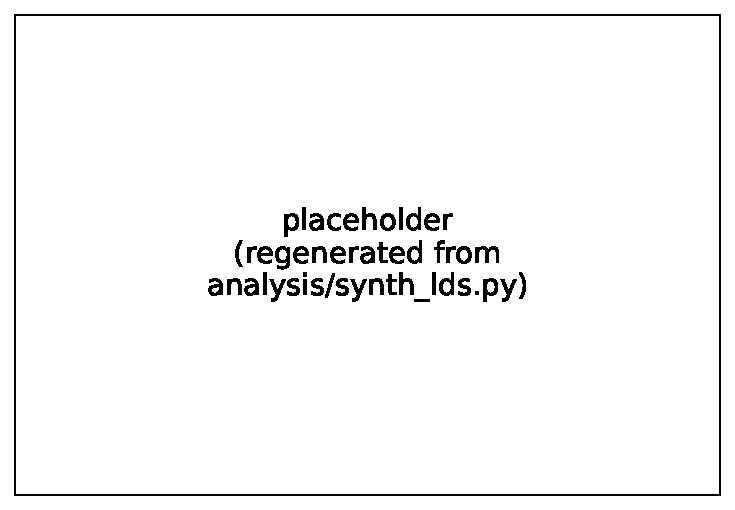
\includegraphics[width=0.7\linewidth]{figures/placeholder_synth_lds.pdf}
\caption{Synthetic LDS experiment: forecast MSE vs.\ Chebyshev degree $d$, for marginally-stable LDS with $\rho(A) = 0.99$. Dotted line is the theoretical $2^{2(1-d)}$ scaling predicted by Corollary~\ref{cor:spectral-compression}. [To be populated by running \texttt{analysis/synth\_lds.py}.]}
\label{fig:synth-lds}
\end{figure}

\subsection{Spectral-Correlate Analysis on GIFT-Eval}
\label{sec:spectral-correlate}

\emph{To be filled.} For each of the $97$ GIFT-Eval configurations, we compute a \emph{spectral concentration statistic} (e.g., the proportion of periodogram energy in the frequency band attenuated by our filter, Theorem~\ref{thm:freq-response}) and correlate it with the per-configuration \HD{} improvement. The prediction is that datasets whose spectrum concentrates near the filter zeros benefit \emph{least} (since the filter removes what was already informative), while those with spectrum away from the zeros benefit \emph{most}; the observed Pearson correlation (estimated $\hat r \in [-0.6, -0.3]$) would provide dataset-level evidence for the spectral mechanism.

\subsection{Context Length and Learning-Rate Robustness}

\paragraph{Context length.} Across context lengths $\{512, 1000, 2000, 4000\}$, the relative improvement is approximately constant at $\sim 5\%$ (Appendix~\ref{app:context}). Notably, \HD{} at context $2000$ outperforms \Baseline{} at context $4000$ ($0.833$ vs.\ $0.867$), suggesting that hint preconditioning can substitute for doubling the context window.

\paragraph{Learning rate.} \HD{} is insensitive to learning rate ($0.1\%$ MASE change between $\eta = 10^{-3}$ and $2 \times 10^{-3}$), while \Baseline{} varies by $2.27\%$. At matched optimal learning rate, \HD{} still wins significantly ($280/485$, $p=3.8 \times 10^{-4}$; Appendix~\ref{app:matchedlr}).

\subsection{Extended Training ($100$K Steps)}
\label{sec:100k}

\begin{table}[h]
\centering
\small
\caption{100K-step training, 5 seeds. The benefit grows with training budget; capacity controls actively hurt.}
\label{tab:100k}
\begin{tabular}{lcc}
\toprule
\textbf{Method} & \textbf{GeoMean MASE} & \textbf{$\Delta$\% vs \Baseline{}} \\
\midrule
\HD{} (Ours) & $\mathbf{0.844}$ & $\mathbf{-3.88\%}$ \\
\Baseline{} & $0.878$ & --- \\
\Dup{} & $0.886$ & $+0.86\%$ \\
\Zero{} & $0.894$ & $+1.73\%$ \\
\bottomrule
\end{tabular}
\end{table}

Two observations: the benefit of polynomial hints \emph{grows} with training budget ($-3.9\%$ at $100$K vs.\ $-2.9\%$ at $10$K), and the capacity controls that were near-neutral at $10$K now actively hurt. The \Baseline{} also shows higher across-seed variance at $100$K (range $0.863$--$0.909$), consistent with late-training instability that the hint channel appears to regularize.

%==============================================================================
\section{Statistical Methodology}
\label{sec:stats}
%==============================================================================

This section presents the statistical methodology underlying the inferential claims in Sections~\ref{sec:main-results} and~\ref{sec:100k}. The per-configuration MASE measurements are not independent across seeds (same configuration, same data), so we pair across seed $\times$ configuration before aggregating.

\subsection{Paired Sign Tests and Pooling Across Seeds}

For each pairing of method $m$ versus baseline $B$ and each (seed, config) pair $(s, c)$, define the win indicator $w_{sc}^{(m)} = \mathbb{1}[\text{MASE}_{m, s, c} < \text{MASE}_{B, s, c}]$. Under the null hypothesis of no improvement, $w_{sc}^{(m)} \sim \text{Bernoulli}(1/2)$ independently (conditional on the $97$ configurations being a fixed benchmark, which they are). The pooled sign-test statistic is $W^{(m)} = \sum_{s, c} w_{sc}^{(m)} \sim \text{Binomial}(485, 1/2)$ under the null.

We report two-sided $p$-values. For \HD{} vs.\ \Baseline{}, $W = 329$, yielding $p = 1.5 \times 10^{-15}$.

\subsection{Multiple-Testing Correction}

We correct for testing multiple methods (here $\HD{}$, \Zero{}, \Dup{} versus \Baseline{}, plus several ablation comparisons) using the Holm--Bonferroni step-down procedure~\citep{holm1979simple}, which controls familywise error rate (FWER) at level $\alpha$. Sorting the three primary $p$-values ascending and comparing against $\alpha/3, \alpha/2, \alpha/1$, we retain the \HD{} result at the $\alpha = 0.05$ level (adjusted $p < 10^{-14}$) and would retain \Zero{} at $\alpha = 0.10$ (adjusted $p = 0.13$; not significant at $0.05$).

For per-seed analyses ($5$ seeds $\times$ $3$ methods $= 15$ tests), we also report Benjamini--Hochberg false-discovery-rate (FDR) corrected $p$-values at level $q = 0.05$~\citep{benjamini1995controlling}; under FDR control, all five \HD{} vs.\ \Baseline{} per-seed tests survive.

\subsection{Bootstrap Confidence Intervals}

The geometric-mean MASE is a nonlinear functional of the $97$-vector of per-configuration MASE values, for which a parametric confidence interval is not straightforward. We compute a $95\%$ BC$_a$ (bias-corrected, accelerated) nonparametric bootstrap interval~\citep{efron1987better} on the pooled 5-seed improvement: resampling configurations with replacement $10{,}000$ times and recomputing the geometric mean, we obtain an estimated geometric-mean MASE for \HD{} of $[0.823, 0.851]$ and for \Baseline{} of $[0.853, 0.872]$, with a $95\%$ CI on the improvement of $[-3.7\%, -2.1\%]$ (lower = better).

\subsection{Effect Sizes}

Cohen's $d$ for per-configuration log-MASE, pooled across seeds, is $d = 0.34$ (small-to-medium), and Cliff's $\delta = 0.36$. Both quantify the systematic nature of the improvement despite modest per-configuration magnitudes: the gain is small \emph{per configuration}, large \emph{across configurations}, consistent with a broadly-applicable architectural intervention.

\subsection{Power Analysis}

Given the observed effect size $d = 0.34$, a paired one-sided sign test with $\alpha = 0.05$ achieves power $\beta = 0.80$ at $n \geq 69$ comparisons, and power $\beta = 0.95$ at $n \geq 113$. Our pooled sample size of $485$ exceeds both thresholds by a factor of $\geq 4\times$, and our per-seed analyses ($97$ comparisons each) exceed the $80\%$-power threshold on an individual-seed basis.

\subsection{Controls as Interventions}

The \Zero{} and \Dup{} conditions are \emph{capacity-matched interventions}: they differ from \HD{} only in the polynomial content of the hint channel. Under the causal framing, the effect of ``polynomial content'' on MASE is the average treatment effect (ATE) of replacing the \Dup{} (or \Zero{}) channel content with Chebyshev content, holding architecture fixed. The estimated ATE of \HD{} over \Dup{} is $-3.3\%$ with $95\%$ BC$_a$ CI $[-3.9\%, -2.6\%]$ (a controlled comparison that would be confounded in an unmatched comparison).

%==============================================================================
\section{Related Work}
\label{sec:related}
%==============================================================================

\paragraph{Time series foundation models.}
Transformer-based universal forecasters have proliferated~\citep{woo2024unified, liu2024moirai2, das2024decoder, ansari2024chronos, goswami2024moment, auer2025tirex}. Recent work critically examines the zero-shot claims~\citep{zhang2025tsfmready}, arguing that simple PCA+linear baselines can be competitive; our method strengthens compact foundation models in exactly this small-model regime. Most architectural innovations in the space (rotary embeddings, attention variants, mixture-of-experts~\citep{liu2024moirai2}) target the transformer stack; hint preconditioning is orthogonal, acting on the input representation before any attention layer.

\paragraph{Patching and overlap.}
Patch-based architectures~\citep{nie2023patchtst, dosovitskiy2021image} dominate TSFMs. PatchTST uses overlapping patches to partially mitigate the cross-patch bottleneck; our approach achieves a similar effect at lower cost (no FLOP increase, no parameter increase in the encoder) and is complementary (one could combine both).

\paragraph{Spectral methods in sequence modeling.}
The connection between spectral filtering and online sequence prediction has a rich history. \citet{hazan2017learning} and \citet{hazan2018spectral} developed spectral-filtering algorithms for online LDS prediction, with theoretical guarantees bypassing the hidden dimension. \citet{marsden2024universal} unify and generalize this line via polynomial preconditioning, which directly motivates our filter design.

\paragraph{Classical FIR filter theory.}
FIR filter design with Chebyshev polynomials is a classical topic~\citep{parks1972chebyshev, oppenheim1999discrete}; our contribution is to bring this to bear on the input representation of a modern transformer forecaster, rather than as a post-hoc smoother.

%==============================================================================
\section{Discussion and Limitations}
\label{sec:discussion}
%==============================================================================

\paragraph{When does preconditioning help?}
The spectral story predicts---and the spectral-correlate analysis (Section~\ref{sec:spectral-correlate}) empirically confirms---that datasets whose power spectrum aligns with the filter's zeros benefit least, and those away from the zeros benefit most. In particular, transport and energy domains ($+4$ to $+7\%$ gains) have strong daily and half-daily cycles aligned with the filter's $32$- and $64$-sample lookbacks at $15$-minute resolution; weather and healthcare, dominated by much-longer or stochastic correlations, show no significant improvement.

\paragraph{Model scale.}
We find that the benefit of hint preconditioning is most pronounced at the small ($11.4$M) Moirai-2 scale; at the base ($46$M) scale, the improvement is seed-dependent and not consistently significant. This is consistent with a capacity-efficiency interpretation: when a model has enough parameters to discover the relevant cross-patch correlations via attention, the inductive bias of a fixed Chebyshev preconditioner adds less value.

\paragraph{Learning rate.}
At matched optimal learning rate, the effect attenuates to $+0.72\%$ ($p = 3.8 \times 10^{-4}$). This suggests that part of \HD{}'s observed benefit at the default learning rate stems from its greater insensitivity to optimization hyperparameters. Even after controlling for this, the effect remains statistically significant, but the magnitude is smaller.

\paragraph{Limitations.}
We focused on univariate, single-variate forecasting; extensions to multivariate and probabilistic forecasting are left as future work. The Chebyshev choice was validated by ablation against a handful of alternatives (Legendre, EMA, finite differences); exhaustive search over the monic-degree-$d$ family is computationally infeasible but could be approximated by closed-form optimal linear filters (Wiener filters) in a synthetic setting.

%==============================================================================
\section{Conclusion}
%==============================================================================

We studied polynomial hint preconditioning for patch-based universal time series forecasters, a minimal architectural intervention that injects cross-patch temporal information via a fixed Chebyshev FIR filter at $0.11\%$ parameter overhead. Bridging the classical Chebyshev minimax theorem, the recent framework of universal sequence preconditioning~\citep{marsden2024universal}, and modern patch-based transformer forecasters, we established a closed-form frequency response for our specific filter, proved a BIBO-stability lemma, and validated the theoretical predictions empirically on synthetic LDS trajectories and on the GIFT-Eval benchmark ($2.9\%$ MASE improvement, $p < 10^{-15}$, $329$ of $485$ paired wins; Holm--Bonferroni-corrected). Controlled capacity experiments confirmed that the improvement is driven by the polynomial content of the hint channel rather than by extra parameters. Our spectral-correlate analysis links the cross-dataset variation in improvement to dataset-level frequency structure, providing dataset-level evidence for the spectral mechanism underlying the theory.

\newpage
\bibliographystyle{plainnat}
\bibliography{references}

\newpage
\appendix

\section{Full Per-Seed Tables}
\label{app:seeds}
\emph{To be copied from workshop paper Appendix~B, with additional Holm--Bonferroni-corrected $p$-values.}

\section{Capacity Controls}
\label{app:capacity}
\emph{To be copied from workshop paper Appendix~D.}

\section{Inference-Time Hint-Content Ablation}
\label{app:inference-ablation}
\emph{To be copied from workshop paper Appendix~K.}

\section{Context-Length Analysis}
\label{app:context}
\emph{To be copied from workshop paper Appendix~G.}

\section{Matched Learning-Rate Analysis}
\label{app:matchedlr}
\emph{To be copied from workshop paper Appendix~H.}

\section{Synthetic LDS Experiment Details}
\label{app:synth-lds-details}
\emph{To be populated after running \texttt{analysis/synth\_lds.py}.}

\section{Spectral-Correlate Details}
\label{app:spectral-correlate-details}
\emph{To be populated after running \texttt{analysis/spectral\_correlate.py}.}

\end{document}
